\begin{frame}
	\titlepage
\end{frame}

\begin{frame}{\S\,5.5\;平面曲线的曲率}
	\linespread{1.5}
	\begin{enumerate}
	  \item {\bf 内容与要求}{\b( 教材上册P120-127 )}
	  \begin{itemize}
	    \item 理解曲率的概念
	    \item 熟练掌握曲率的计算公式
	    \item 了解曲率的应用
	  \vspace{1em}
	  \end{itemize}
	  \item {\bf 课后练习:}
	  \begin{itemize}
	    \item {\b 习题5.5:5,6,7,8,11}
	  \end{itemize}
	\end{enumerate}
\end{frame}

% \begin{frame}
% 	\tableofcontents
% \end{frame}

\begin{frame}{复习与回顾}
	\linespread{1.5}
	\ba{如何刻画一条平面曲线的几何特征?}
	
% 	设$y=f(x)$表示平面上一条曲线,则
	\begin{enumerate}
	  \item {\bf 切线斜率:}一阶导数
	  \item {\bf 凹凸性:}二阶导数
	  \item {\bf 长度:}弧微分
	  \item {\bf 弯曲程度:}{\b 曲率}
	\end{enumerate}
\end{frame}

\section{曲率的概念}

\begin{frame}{曲率}
	\linespread{1.2}
	\centerline{\ba{如何刻画曲线的弯曲程度?}}\pause 
	\begin{columns}
		\column{.5\textwidth}
			\begin{center}
				\resizebox{!}{3.8cm}{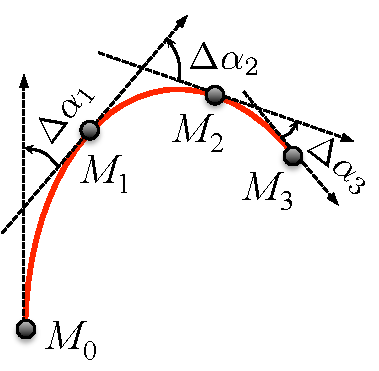
\includegraphics{./images/lineAngle.pdf}}
				
				\pause {\b 长度相同的曲线,
				
				转角越大弯曲程度越大}\pause 
			\end{center}
		\column{.5\textwidth}
			\begin{center}
				\resizebox{!}{3.8cm}{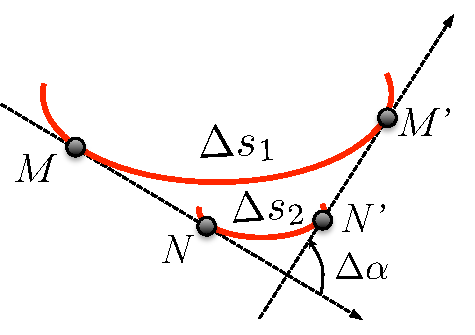
\includegraphics{./images/angleLine.pdf}}
				
				\pause {\b 转角相同的曲线,
				
				弧长越短弯曲程度越大}
			\end{center}
	\end{columns}
\end{frame}

% \begin{frame}{弧微分}\pause 
% 	\linespread{1.2}
% % 	{\bf 问题:}如何定量刻画曲线弯曲的程度?\\
% 	{\bb 弧微分:}曲线$y=f(x)$的弧长关于自变量$x$的微分\pause 
% 	$$ds=\sqrt{1+(y')^2}dx\pause =\sqrt{(dx)^2+(dy)^2}$$\pause 
% 	\vspace{-1em}
% 	\begin{itemize}
% 	  \item 参数方程形式\pause 
% 	  $$ds=\sqrt{[x'(t)]^2+[y'(t)]^2}dt$$\pause 
% 	  \vspace{-3ex}
% 	  \item 极坐标形式\pause 
% 	  $$ds=\sqrt{\rho^2(\theta)+[\rho'(\theta)]^2}d\theta$$
% 	\end{itemize}
% \end{frame}

\begin{frame}
	\linespread{1.5}
	\ba{曲线的弯曲程度与切线的转角成正比,弧长成反比}\pause
	\begin{block}{{\bf 定义5.5.1}\hfill P285}
	\begin{columns}
		\column{.6\textwidth}
			设曲线$C:y=f(x)$光滑,	以$M_0$为基点,到曲线上另一点$M$的弧长
			为$\Delta s$,切线转角为$\Delta\alpha$,若极限$\lim\limits_{\Delta s\to
			0}\left|\df{\Delta\alpha}{\Delta s}\right|$存在,
			则称之为{\bb 曲线$C$在$M_0$处的曲率},记为
		\column{.4\textwidth}
			\begin{center}
				\resizebox{!}{4cm}{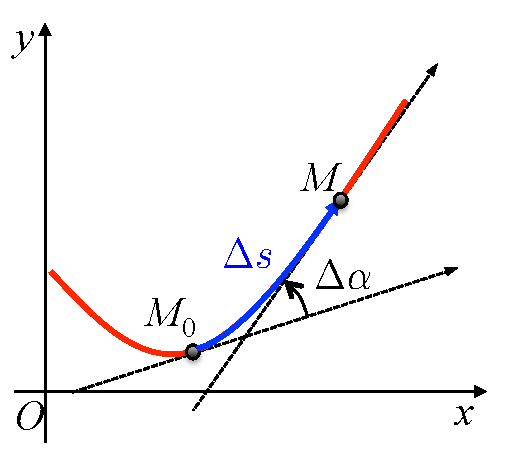
\includegraphics{./images/def.pdf}}
			\end{center}
	\end{columns}\pause 
	$$\alert{K=\lim\limits_{\Delta s\to
				0}\left|\df{\Delta\alpha}{\Delta s}\right|\pause
				=\left|\df{d\alpha}{ds}\right|}$$ 
	\end{block}
% 	\pause 
% 	\begin{itemize}
% 	  \item 切线角度相对于弧长的变化率的绝对值
% 	\end{itemize}
% 	\begin{exampleblock}{{\bf 例2}\hfill P286-例2}
% 		求直线和圆的曲率.
% 	\end{exampleblock}
\end{frame}

\begin{frame}
	\linespread{1.2} 
	$$\alert{K=\lim\limits_{\Delta s\to
				0}\left|\df{\Delta\alpha}{\Delta s}\right|
				=\left|\df{d\alpha}{ds}\right|}$$ 
% 	{\bb 曲率:}与局部的转角成正比,弧长成反比
% 	\begin{block}{{\bf 定义5.5.1}\hfill P285}
% 		切线角度相对于弧长的变化率的绝对值\pause 
% 		$$K=\left|\df{d\alpha}{ds}\right|\pause =\lim\limits_{\Delta x\to
% 		0}\left|\df{\Delta\alpha}{\Delta s}\right|$$
% 	\end{block}\pause 
	\pause 
	\begin{exampleblock}{{\bf 例1}\hfill P286-例2}
		求直线上任一点处的曲率。
	\end{exampleblock}
	\pause {\bf 解:}直线上任一点处的切线就是直线本身\pause ,故其上任意两点之间的线段上
	的切线转角$\Delta\alpha=0$,\pause 从而
	$$K=\lim\limits_{\Delta s\to 0}\left|
	\df{\Delta\alpha}{\Delta s}\right|=0.$$
	\vspace{-1em}
	\begin{itemize}\pause 
	  \item \ba{$K=0$:直线不弯曲!}
	\end{itemize}
\end{frame}

\begin{frame}
	\linespread{1.2}
% 	$$\alert{K=\lim\limits_{\Delta s\to
% 				0}\left|\df{\Delta\alpha}{\Delta s}\right|\pause
% 				=\left|\df{d\alpha}{ds}\right|}$$ 
	\begin{exampleblock}{{\bf 例2}\hfill P286-例2}
		求半径为$R$的圆上任一点处的曲率。
	\end{exampleblock}
	\pause 
	\begin{columns}
		\column{.7\textwidth}
			\begin{center}
				\resizebox{!}{4.5cm}{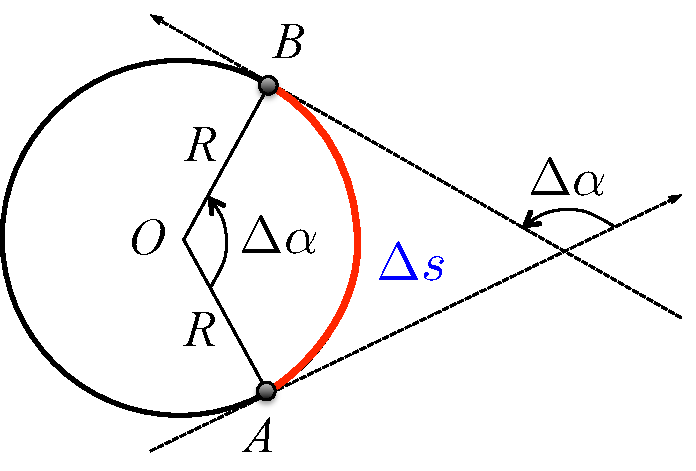
\includegraphics{./images/sphere.pdf}}
			\end{center}
		\column{.3\textwidth}\pause 
			$$\alert{K=\df 1R}$$
	\end{columns}
	\begin{itemize}\pause 
	  \item \ba{圆上每一点处曲率相同}\pause 
	  \item \ba{圆的半径越小,曲率越大}
	\end{itemize}
\end{frame}

\section{曲率的计算}

\begin{frame}{曲率的计算}
	\linespread{1.2}\pause 
	设$y=f(x)$二阶可导,则
	\alert{$$K=\df{|y''|}{[1+(y')^2]^{3/2}}$$}\pause 
	\begin{exampleblock}{{\bf 例3}\hfill P287-例5}
		抛物线$y=ax^2+bx+c$在哪一点的曲率最大?
	\end{exampleblock}\pause 
% 	$$K=\df{|2a|}{[1+(2ax+b)^2]^{3/2}}$$
	\begin{itemize}
	  \item \ba{抛物线在顶点处的曲率最大}
	\end{itemize}
\end{frame}

% \begin{frame}
% 	\linespread{1.2}\pause 
% 	\alert{$$K=\df{|y''|}{[1+(y')^2]^{3/2}}$$}\pause 
% 	\begin{exampleblock}{{\bf 例3}\hfill P287-例5}
% 		我国铁路常用立方抛物线$y=\df 1{6Rl}x^3$作为缓和曲线,其中
% 		$R$是圆弧弯道的半径,$l$是缓和曲线的长度,且$l<<R$,求缓和曲线
% 		两端点$O(0,0)$和$B(l,l^2/(6R))$处的曲率。
% 	\end{exampleblock}
% 	{\bf 说明:}铁路转弯时为保证列车平稳安全,离心力必须
% 	  连续变化,因此铁道的曲率应该是连续变化的。
% \end{frame}

\begin{frame}
	\linespread{1.2}
	\alert{{\bf 说明:}根据不同形式的曲线方程,可以得到相应的曲率公式}\pause 
	\begin{enumerate}
	  \item 若曲线由参数方程$\left\{\begin{array}{l}
	  x=\varphi(t)\\ y=\psi(t)
	  \end{array}\right.$给出,\pause 则
	  $$\alert{K=\df{|\varphi'(t)\psi''(t)-\varphi''(t)\psi'(t)|}
		{\{[\varphi'(t)]^2+[\psi'(t)]^2\}^{3/2}}}$$\pause 
	  \item 若曲线方程为$x=g(y)$,\pause 则
		$$\alert{K=\df{|g''(y)|}{\{[1+[g'(y)]^2\}^{3/2}}}$$
	\end{enumerate}
% 	设$x=\varphi(t),y=\psi(t)$二阶可导,则
% 	\alert{$$K=\df{|\varphi'(t)\psi''(t)-\varphi''(t)\psi'(t)|}
% 	{\{[\varphi'(t)]^2+[\psi'^2(t)]^2\}^{3/2}}$$}\pause 
% 	\begin{exampleblock}{{\bf 例3}\hfill P287-例5}
% 		求椭圆$\left\{\begin{array}{l}
% 		x=a\cos t\\ y=b\sin t
% 		\end{array}\right.(0\leq t\leq \pi)$在何处曲率最大?
% 	\end{exampleblock}
% 	{\bf 结论:}设$0<b<a$,则椭圆在$(\pm a,0)$处曲率最大。
\end{frame}

% \begin{frame}{参数方程下的曲率计算}
% 	\linespread{1.2}\pause 
% 	设$x=\varphi(t),y=\psi(t)$二阶可导,则
% 	\alert{$$K=\df{|\varphi'(t)\psi''(t)-\varphi''(t)\psi'(t)|}
% 	{\{[\varphi'(t)]^2+[\psi'^2(t)]^2\}^{3/2}}$$}\pause 
% 	\begin{exampleblock}{{\bf 例3}\hfill P287-例5}
% 		求椭圆$\left\{\begin{array}{l}
% 		x=a\cos t\\ y=b\sin t
% 		\end{array}\right.(0\leq t\leq \pi)$在何处曲率最大?
% 	\end{exampleblock}
% 	{\bf 结论:}设$0<b<a$,则椭圆在$(\pm a,0)$处曲率最大。
% \end{frame}

% \begin{frame}{参数方程下的曲率计算}
% 	\linespread{1.2}\pause 
% 	设$x=\varphi(t),y=\psi(t)$二阶可导,则
% 	\alert{$$K=\df{|\varphi'(t)\psi''(t)-\varphi''(t)\psi'(t)|}
% 	{\{[\varphi'(t)]^2+[\psi'^2(t)]^2\}^{3/2}}$$}\pause 
% 	\begin{exampleblock}{{\bf 例3}\hfill P287-例5}
% 		求圆滚线
% 		$$\left\{\begin{array}{l}
% 		x=a(t-\sin t)\\
% 		y=a(1-\cos t)
% 		\end{array}\right.\quad (a>0)$$
% 		在$(\pi a,2a)$处的曲率。
% 	\end{exampleblock}
% \end{frame}

\section{曲率半径与曲率圆}

\begin{frame}{曲率半径与曲率圆}
	\linespread{1.2} 
	\begin{block}{\bf 定义}
	\begin{columns}[t]
		\column{.6\textwidth}\pause 
			\begin{enumerate}
			  \item {\bb 曲率半径:} $R=\df 1K$\pause 
			  \item {\bb 曲率中心:}曲线凹一侧法线上,距离切点为$R$的点\pause 
			  \item {\bb 曲率圆:}以$D$为圆心,$R$为半径的圆\pause 
			\end{enumerate}
		\column{.4\textwidth}
			\vspace{-3ex}
			\begin{center}
				\resizebox{!}{3.4cm}{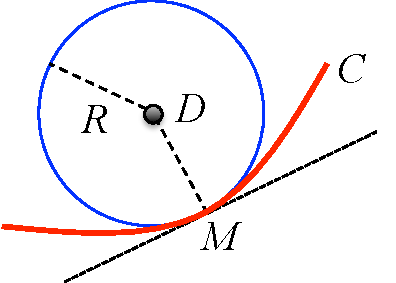
\includegraphics{./images/curSphere.pdf}}
			\end{center}
% 			\bigskip
	\end{columns}
	\end{block} 
	\begin{itemize}\pause 
	  \item \alert{曲率圆与已知曲线在切点处曲率相同}\pause 
	  \item \alert{曲率圆与已知曲线二阶相切}
	\end{itemize}
\end{frame}

% \begin{frame}{曲率半径与曲率圆}
% 	\linespread{1.5}\pause 
% 	{\bb 曲率半径:}\pause $R=\df 1K$\\ \pause 
% 	{\bb 曲率圆:}\pause 曲线凹一侧,以$R$为半径,与曲线相切的圆\\ \pause 
% 	{\bb 曲线的$n$阶相切:}\pause 曲线$y=\varphi(x)$和$y=\psi(x)$满足\pause 
% 	$$\varphi^{(k)}(x_0)=\psi^{(k)}(x_0),\;k=0,1,2,\ldots,n$$\pause 
% 	且
% 	$$\varphi^{(n+1)}(x_0)\ne\psi^{(n+1)}(x_0)$$
% 	%画图,标记
% \end{frame}

% \begin{frame}{曲率半径与曲率圆}
% 	\linespread{1.5}\pause 
% 	{\bb 曲率半径:}\pause $R=\df 1K$\\ \pause 
% 	{\bb 曲率圆:}\pause 曲线凹一侧,以$R$为半径,与曲线相切的圆\\ \pause 
% 	{\bb 曲线的$n$阶相切:}\pause 曲线$y=\varphi(x)$和$y=\psi(x)$满足\pause 
% 	$$\varphi^{(k)}(x_0)=\psi^{(k)}(x_0),\;k=0,1,2,\ldots,n$$\pause 
% 	且
% 	$$\varphi^{(n+1)}(x_0)\ne\psi^{(n+1)}(x_0)$$
% \end{frame}

% \begin{frame}{曲率圆}
% 	\linespread{1.5}\pause 
% 	{\bb 曲率圆:}与原曲线二阶相切的圆\\ \pause 
% 	给定曲线$y=f(x)$,设$f''(x)>0$,其{\bb 曲率圆方程}:\pause 
% 	$$(x-\xi)^2+(y-\eta)^2=R^2$$
% 	其中:
% 	$$\xi=x-\df{y'[1+(y')^2]}{y''},\quad \eta=y+\df{1+(y')^2}{y''}$$
% \end{frame}

\begin{frame}
	\linespread{1.5} 
	\begin{exampleblock}{{\bf 例4}\hfill P287-例5}
		设一工件某侧的截痕为抛物线$y=ax^2+bx+c$,现要用圆形砂轮打磨其表面,
		问该如何选择砂轮的尺寸?
	\end{exampleblock}
	\pause 
	\begin{center}
		\resizebox{!}{5.5cm}{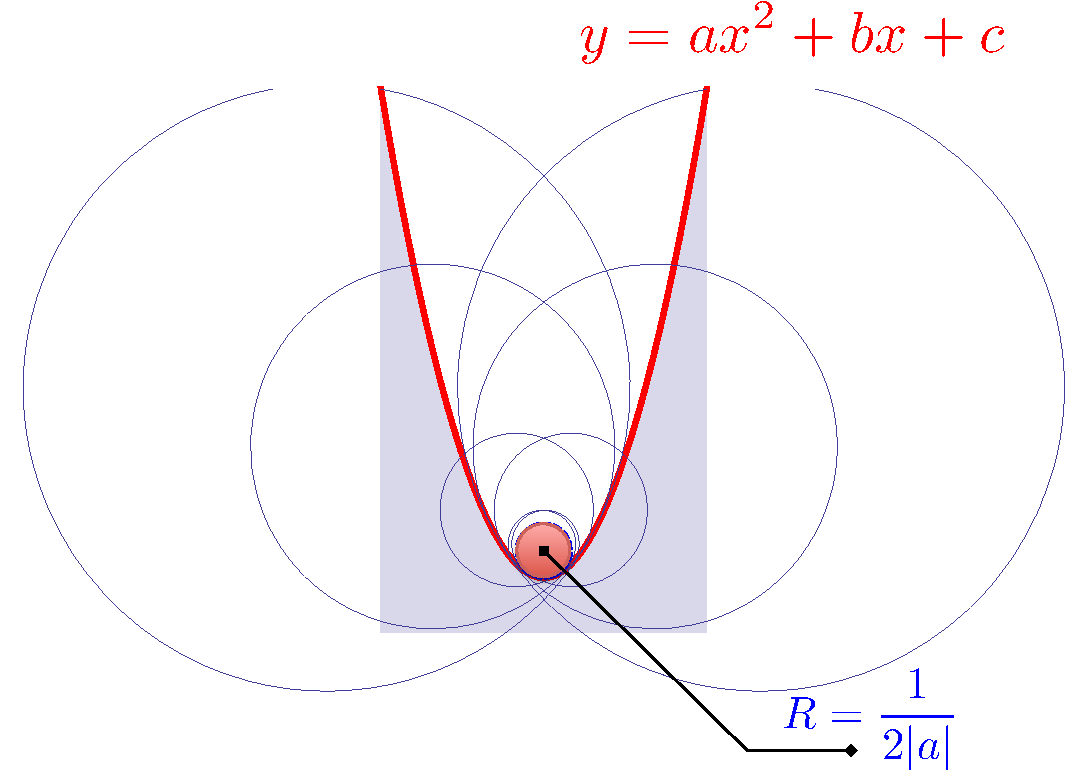
\includegraphics{./images/curlingR.pdf}}
	\end{center}
\end{frame}

\section{曲率的应用}

\begin{frame}{离心力与曲率半径}
	\linespread{1.2}
	\begin{columns}
		\column{.6\textwidth}
			质量为$m$的质点以速度$v$通过光滑曲线上一点,所受离心力为
			$$F=\df{mv^2}{R},$$
			其中$R$为曲线在该点处的曲率半径。
		\column{.4\textwidth}
			\begin{center}
				\resizebox{!}{4.5cm}{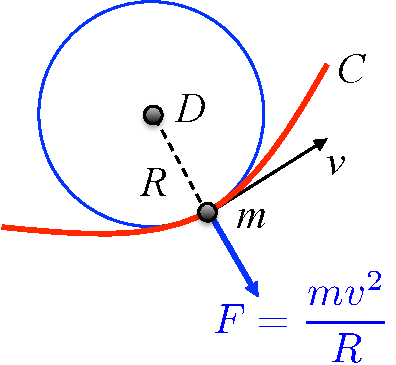
\includegraphics{./images/flip.pdf}}
			\end{center}
	\end{columns}
\end{frame}

\begin{frame}{铁路中的缓和曲线}
	\linespread{1.2}\pause 
	\ba{为了确保列车行驶安全,连接直线和圆弧轨道的路段应该尽可能保证列车运行时所受离心力的平稳变化}\pause 
	\begin{center}
		\resizebox{!}{5.5cm}{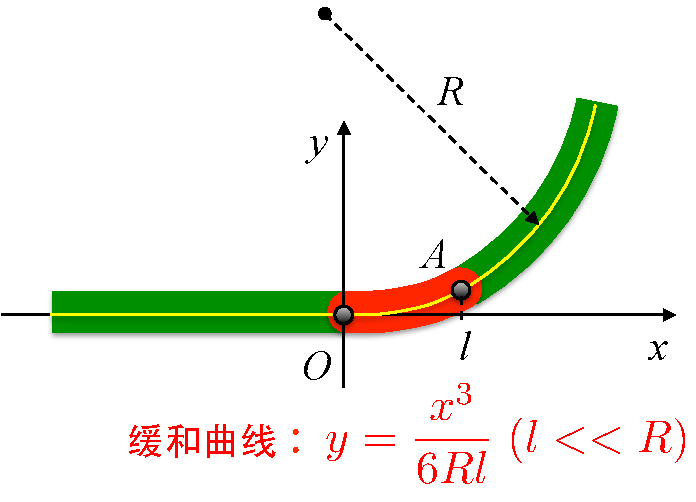
\includegraphics{./images/releaseCurve.pdf}}
	\end{center}
\end{frame}

\begin{frame}[<+->]{小结}
	\linespread{1.5}
	\begin{enumerate}
	  \item {\bf 曲率:}切线转角关于弧长的相对变化率
	  \item {\bf 曲率的计算:}
	  \begin{itemize}
	    \item 对应于各种不同的曲线方程的曲率公式
	  \end{itemize}
	  \item {\bf 曲率半径与曲率圆:}
	  \begin{itemize}
	    \item 离心力与缓和曲线
	  \end{itemize}
	\end{enumerate}
	\begin{block}{{\bf 课后练习}\hfill}
		{\b\quad 习题5.5:5,6,7,8,11}
	\end{block}
\end{frame}

%===============================

% \begin{frame}{title}
% 	\linespread{1.2}
% 	\begin{block}{{\bf title}\hfill}
% 		123
% 	\end{block}
% \end{frame}